\documentclass[11pt,a4paper]{article}

\usepackage{style2017}
\usepackage{hyperref}
\usepackage{pifont}
\usepackage{subcaption}

\hypersetup{
    colorlinks =false,
    linkcolor=blue,
   linkbordercolor = 1 0 0
}
\newcounter{numexo}
\setcellgapes{1pt}

\newcommand{\nd}{n\oe{}ud~}
\newcommand{\Nd}{N\oe{}ud~}
\newcommand{\nds}{n\oe{}uds~}

\setlength{\parskip}{0.5em}

\lstset{%
	language={python},
	frame=single,
	xleftmargin=2cm,
	xrightmargin=2cm,
	basicstyle = \ttfamily,
	breaklines=true,
	%numbers=left,
	numberstyle=\footnotesize,
	captionpos=b,
	basicstyle=\ttfamily,
	keywordstyle=\bfseries\color{blue},
	commentstyle=\itshape\color{green},
	moredelim=[il][\color{red}]{/+},%
	}
	
\begin{document}

\begin{NSI}
{Activité}{Algorithme des k plus proches voisins}
\end{NSI}

L'algorithme des k plus proches voisins (de l'anglais \textit{k-nearest-neighbors} abrégé en kNN) est un algorithme simple d'apprentissage utilisé en \textit{machine learning}. Il permet de classifier un jeu de données selon un critère précis, comme par exemple, répondre Oui ou Non à une question ou encore indiquer si une image représente un chien ou un chat.


\subsection*{Présentation du problème}

En 1936, le statisticien britannique Ronald Fisher a utilisé un jeu de données basé sur 150 fleurs d'iris, appartenant à 3 variétés différentes : Setosa, Versicolor et Virginica. Il souhaitait pouvoir déterminer la variété d'une fleur d'iris prélevée au hasard dans la nature.

\begin{figure}[h]
  \centering
  \begin{subfigure}[b]{0.17\textwidth}
     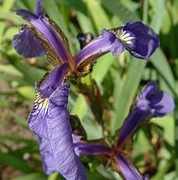
\includegraphics[scale=0.5]{img/Iris_setosa_1.jpg}
     \caption{Iris Setosa}
     \label{fig:edge-a}
  \end{subfigure}
  \begin{subfigure}[b]{0.275\textwidth}
     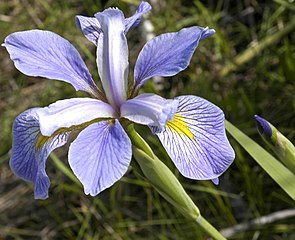
\includegraphics[scale=0.5]{img/Iris_virginica_1.jpg}
     \caption{Iris Virginica}
     \label{fig:contour-b}
  \end{subfigure}
  \begin{subfigure}[b]{0.27\textwidth}
     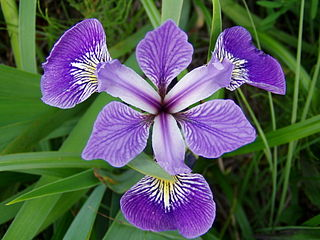
\includegraphics[scale=1]{img/Iris_versicolor_1.jpg}
     \caption{Iris Versicolor}
     \label{fig:contour-c}
  \end{subfigure}
\end{figure}

\begin{enumerate}
\item En examinant seulement les photos ci-dessus, donner quelques critères discriminants qui permettraient de classifier les fleurs d'iris.
\vspace{3cm}
\item En vous aidant de la photo ci-dessous, préciser quelles sont les caractéristiques des fleurs mesurées par Fisher.

\begin{figure}[h]
  \centering
  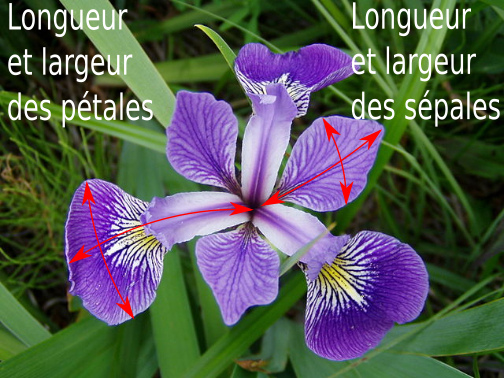
\includegraphics[scale=0.5]{img/Iris_mesure.png}    
\end{figure}
\end{enumerate}

\vspace{2cm}

\newpage
\subsection*{Étude du problème à résoudre}


Le fichier \textsf{iris.csv} contient les relevés des 150 iris effectués par Ronald Fisher. Vous trouverez ce fichier sur l'ENT dans la parie \textbf{Algorithme des plus proches voisins} (moodle).

L'objectif de cette partie est d'exploiter et représenter graphiquement ce jeu de données en Python.

On rappelle quelques fonctions qui seront utiles à l'écriture de notre script.

\begin{itemize}
\item \textsf{with open("iris.csv",mode='r',encoding='utf8',newline='') as f:} permet d'ouvrir un fichier en lecture pour en extraire les données. Ici l'ouverture se fait avec l'alias \textsf{f}.
\item \textsf{data = csv.reader(f,delimiter=',')} permet de transformer les données du fichier \textsf{csv} en listes.
\item \textsf{from matplotlib import pyplot} pour importer le module \textsf{pyplot} du module \textsf{matplotlib}.
\item \textsf{pyplot.scatter(x, y, c='couleur')} pour placer les points de coordonnées $(x;y)$. Les arguments \textsf{x} et \textsf{y} sont des listes de valeurs ou des nombres entiers représentant les abscisses et les ordonnées des points.
\end{itemize}

\begin{enumerate}
\item En utilisant le module \textsf{csv}, ouvrir en lecture le fichier \textsf{iris.csv} et rassembler les données de chaque fleur dans une liste. Au final, on obtient 150 listes de 5 valeurs \textsf{['ID', 'SeL', 'SeW', 'PeL', 'PeW']}.
\item Compléter votre code pour rassembler dans une même liste \textsf{variete} la variété des 150 iris : \textsf{setosa}, \textsf{virginica} et \textsf{versicolor}.
\item Compléter votre code pour rassembler dans une même liste \textsf{sew} les 150 mesures \textsf{SeW} indiquant la largeur des sépales.
\item Compléter votre code pour rassembler dans une même liste \textsf{pew} les 150 mesures \textsf{PeW} indiquant la largeur des pétales.
\item Représenter avec le module \textsf{pyplot} les points représentant les iris en prenant pour abscisse la largeur des sépales et en ordonnée la longueur des pétales.

On doit obtenir le graphique suivant:
\begin{center}
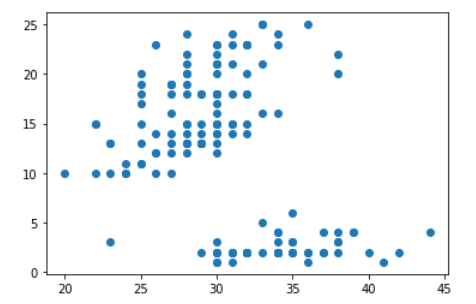
\includegraphics[scale=0.8]{img/graphique_1.png}
\end{center}
\item On veut colorer les points selon la variété des iris. Les points représentant les \textbf{setosa} seront en orange, les \textbf{virginica} en bleu et les \textbf{versicolor} en vert.

Modifier votre script avec une boucle \textsf{for} pour donner la bonne couleur au point représentant la variété d'iris. On doit obtenir le graphique suivant:
\begin{center}
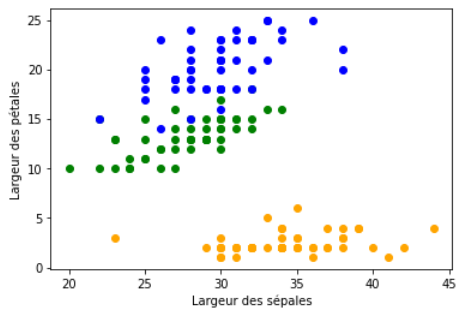
\includegraphics[scale=0.8]{img/graphique_2.png}
\end{center}



\item Que remarque-ton sur le graphique concernant une même variété d'iris ?
\vspace{2cm}

\item Comment exploiter ce graphique pour déterminer la variété d'une fleur d'iris trouvée en pleine nature ? Préciser en particulier le rôle joué par les k plus proches voisins.
\vspace{2cm}

\item On suppose que vous trouvez dans la nature les trois fleurs d'iris dont les mesures sont les suivantes:\medskip

\renewcommand{\arraystretch}{1.2}
\begin{tabular}{*{6}{|C{2.5cm}}|}\hline
Fleur d'iris à classifier & Longueur du sépale (en cm) &  Largeur du sépale (en cm) &  Longueur du pétale (en cm) &  Largeur du pétale (en cm) & Classe d'iris\\\hline
1 & 5,1 & 3,5 & 1,4 & 0,2 & \\\hline
2 & 6,4 & 3,0 & 4,5 & 1,4 & \\\hline
3 & 5,9 & 3,0 & 5,0 & 1,8 & \\\hline
\end{tabular}

\begin{enumerate}
\item Placer sur le graphique précédent les trois nouvelles fleurs d'iris inconnues.
\item Attribuer à chacun de ces iris sa classe ou variété.
\end{enumerate}

\end{enumerate}

\newpage
\subsection*{Recherche d'un algorithme de classification}

L'algorithme kNN permet de prédire la classe (variété) du sujet à étudier en fonction de ses k plus proches voisins. L'entier k doit être optimisé pour chaque étude. Une bonne méthode consiste à prendre $k=\sqrt{n}$ où $n$ est le nombre de sujets étudiés dans la base de départ.

\begin{enumerate}
\item Déterminer la valeur de $k$ à retenir dans notre étude des iris. Comment se calcule cette valeur en Python?
\vspace{2cm}

\item Pour connaître les $k$ plus proches voisins, il faut calculer les distances euclidiennes entre le sujet étudié (nouvel iris) et les points de la base de départ (150 iris).

Quelle est la formule qui permet de calculer cette distance entre deux points $A(x_{A};y_{A})$ et $B(x_{B};y_{B})$ .
\vspace{2cm}

\item Écrire, en Python, une une fonction \textsf{distance(xA,yA,xB,yB)} qui calcule la distance euclidienne entre les deux points A et B.

\item Écrire en Python, la fonction \textsf{kNN(liste,x,y,k)} qui renvoie la classe (variété) d'une fleur d'iris en fonction de la classe majoritaire de ses $k$ plus proches voisins. Cette fonction remplira les conditions suivantes:

\begin{itemize}
\item Le paramètre \textsf{liste} contient les 150 iris de la base Fischer. Chaque valeur (iris) de cette liste est de la forme \textsf{[sew,pew,variété]}.

\item Une fois la distance calculée entre le nouvel iris et un iris de la base, on ajoute dans une liste \textsf{distance\_variete} la distance calculée et la variété du lys de base. Cette liste sera triée par ordre croissant selon les distances euclidiennes.

\item Pour finir, on détermine la variété majoritaire parmi les $k$ premiers éléments de la liste.

\item La fonction renvoie la classe majoritaire trouvée.
\end{itemize}

\item Tester votre fonction avec les trois nouveaux iris donnés dans le tableau précédent.
\end{enumerate}

\end{document}
